%%%%%%%%%%%%%%%%%%%%%%%%%%%%%
%%% - Team Organization - %%%
%%%%%%%%%%%%%%%%%%%%%%%%%%%%%
\subsection{Team Organization}
\label{ssec:TeamOrganization}

%Team Organization Chart:
\begin{wrapfigure}[7]{R}{0in}
	\centering
	\raisebox{0pt}[\dimexpr\height-3\baselineskip\relax]{
		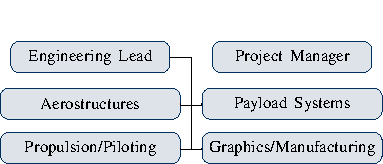
\includegraphics[]{team_organization_chart.pdf}}
	\caption{Here we show the structure of, and assignment areas within, our team organization.}
	\label{fig:personnelassignments}
\end{wrapfigure}
%%%TEAM ORGANIZATION
%\begin{wrapfigure}[7]{R}{0in}
%	\centering
%	\raisebox{0pt}[\dimexpr\height-3\baselineskip\relax]{
\documentclass[]{../byu-aero}

\usepackage[active,tightpage]{preview}
\PreviewEnvironment{tikzpicture}
\setlength{\PreviewBorder}{0em}

\tikzstyle{block1} = [rectangle, draw=\BYUblue, fill=\BYUbluelite, text width=1.35cm, text centered, rounded corners, minimum height=2.5em]

\tikzstyle{arrowblue} = [->,>=stealth,draw=\BYUblue]
\tikzstyle{arrowred} = [->,>=stealth,draw=\BYUred]


\begin{document}

\spacing{.8}
\begin{tikzpicture}[node distance = 0.5cm, auto]

	% Place nodes
	\node [minimum width=1cm] (Advisor) {BYU DBF Team};
	
	\node [block1, below left = 0.15cm and -1.0cm  of Advisor] (Engineering Lead) {\footnotesize Engineering\\Lead};
	\node [block1,draw=\BYUred, below right = 0.15cm and -1.0cm   of Advisor] (Project Manager) {\footnotesize Project\\Manager};

	\node [block, below = 1.25cm of Advisor] (Aerostructures) {\footnotesize Aerostructures};

	\node [block, below = 1.95cm of Advisor] (Propulsion/Piloting) {\footnotesize Propulsion/Piloting};
	
	\node [block, below  = 2.65cm of Advisor] (Payload Systems) {\footnotesize Payload Systems};
	
	\node [block, below  = 3.35cm of Advisor] (Graphics/Manufacturing) {\footnotesize Graphics/Manufacturing};
	

	
	
	\draw[arrowred] (Engineering Lead) -- (Project Manager);
	\draw[arrowred] (Aerostructures) --  ++(2.125cm,0) |- (Project Manager);
	\draw[arrowred] (Propulsion/Piloting) --  ++(2.125cm,0) |- (Project Manager);
	\draw[arrowred] (Payload Systems) --  ++(2.125cm,0) |- (Project Manager);
	\draw[arrowred] (Graphics/Manufacturing) --  ++(2.125cm,0) |- (Project Manager);
	
		\draw[arrowblue] (Aerostructures) --  ++(-2.125cm,0) |- (Engineering Lead);
	\draw[arrowblue] (Propulsion/Piloting) --  ++(-2.125cm,0) |- (Engineering Lead);
	\draw[arrowblue] (Payload Systems) --  ++(-2.125cm,0) |- (Engineering Lead);
	\draw[arrowblue] (Graphics/Manufacturing) --  ++(-2.125cm,0) |- (Engineering Lead);





	\draw[draw=\BYUblue, rounded corners] ($(current bounding box.south east)+(6pt,-6pt)$) rectangle ($(current bounding box.north west)+(-6pt,6pt)$);
	
\end{tikzpicture}%}
%	\caption{Here we show the structure of, and assignment areas within, our team organization.}
%	\label{fig:personnelassignments}
%\end{wrapfigure}

\end{document} %You can change the team_organization.tex file to update this and it will automatically update in this file.


%Introduction
\Cref{fig:personnelassignments} depicts the overall organization of our team structure.  Each of the teams is lead by an individual who answers to the Engineering Lead and Project Manager.  The skills required for each position/team are as follows.




%Team role descriptions continued.
\subsubsection{Engineering Lead} As with the team leads, the Engineering Lead primarily requires good decision making and leadership skills, qualities the BYU Aero Club seeks to develop in all of its members.
In addition the Engineering Lead has a well rounded understanding of the various systems and both design and testing expertise.
%schedule/milestone chart (since it fits here better.)  Note that you must modify this in the ganttchart.tex file, compile that file, and then compile this file again if you change the schedule.


\subsubsection{Project Manager}\begin{wrapfigure}[13]{R}{0pt}
		\raisebox{0pt}[\dimexpr\height-2\baselineskip\relax]{
	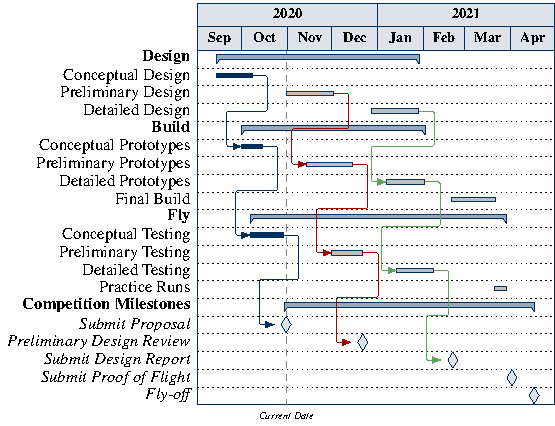
\includegraphics[width=0.45\textwidth]{ganttchart.pdf}}
	\caption{Our {\color{\BYUblue} Conceptual}, {\color{\BYUred} Preliminary}, and {\color{\BYUgreen} Detailed} design phases all culminate in internal design reviews, in addition to the required submissions.}
	\label{fig:plannedtiming}
\end{wrapfigure} The Project Manager has excellent organizational skills
and oversees the logistical side of the project: heading up report writing, budgeting tasks, scheduling, etc.
\subsubsection{Aerodynamics} The Aerodyanmics team members have expertise in aerodynamic analysis and testing, including skills in hand calculations, computational analysis tools, wind tunnel and glide testing.
\subsubsection{Structures} The Structures team members focus on skills in structural analysis and testing, employing hand calculations, computational tools, and various structural testing methods.
\subsubsection{Propulsion} The Propulsion team focuses on analyzing and testing the propulsion system effectiveness and efficiency, but also has skills in electronics related to the propulsion system.
\subsubsection{Systems} The Systems team works very closely with the Engineering Lead, as they oversee all systems interfacing, avionics, etc.  There is a sub-group of the Systems team that is assigned to work on the mission specific payload and related components, as well as related testing. %TODO: consider updating this sentence to reflect the actual specialized mission requirements for the year.
\subsubsection{Manufacturing} The Manufacturing team oversees the manufacturing of all prototypes and testing apparatus.
\subsubsection{Graphics} The Graphics team has skills in CAD design as well as graphical marketing for the team. 